\newpage
\section{LSB}
La technique de stéganographie LSB, pour least significant bit, est une méthode pour cacher des données que ce soit du texte, une image ou tout autre fichier dans une image en utilisant le bit de poids faible des octets représentant chaque pixel.
\newline
Cette technique ne comporte pas beaucoup de limitations ci ce n'est d'avoir une donnée à cacher d'une taille maximale en bits de 3/8 du nombre de pixels composant l'image au format PNG-8 (j'explique à la section x.x quelles en sont les raisons).

\subsection{Format PNG}
Pour illustrer cette technique de stéganographie, je vais utiliser le format d'image PNG avec une taille de canal de couleur sur 8 bits.

\subsubsection{Qu'est-ce que le format PNG ?}
Le format PNG a été créé dans le but de compenser les limitations du format GIF (format propriétaire) tout en le rendant beaucoup plus simple à implémenter. Il représente ses pixels sous forme matriciel avec 3 canaux de couleurs RVB.

\subsubsection{Chunks}
Le format PNG est composé d'un magic number et de multiples chunks. Un chunk est une structure permettant de décrire les différentes données d'un fichier PNG. Chaque chunk est composé de 4 parties :
\paragraph{Longueur}
Sur 4 octets et peut être 0, spécifie la taille que prend la section données du chunk.
\paragraph{Type}
Sur 4 octets, spécifie le type du chunk (exemple : IDAT, IEND, etc.).
\paragraph{Données}
De la taille spécifiée dans la section longueur, contient les données de ce chunk.
\paragraph{CRC}
Checksum de l'intégrité de la section données.

\subsection{Structure du format PNG}
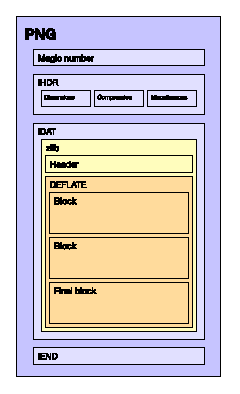
\includegraphics[width=1\textwidth]{img/png-file-format.eps}

\subsubsection{PNG file signature/magic number}
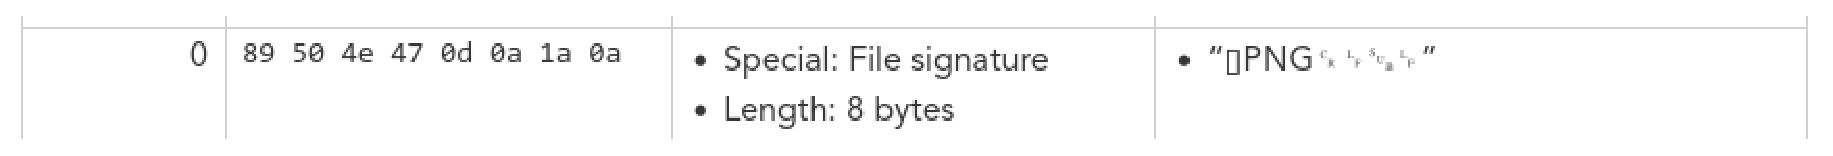
\includegraphics[width=1\textwidth]{img/png_magic_number.eps}
Suite de 8 octets permettant de reconnaitre le format de fichier PNG. Cette suite est celle-ci : 137 80 78 71 13 10 26 10


\subsubsection{IHDR image header chunk}
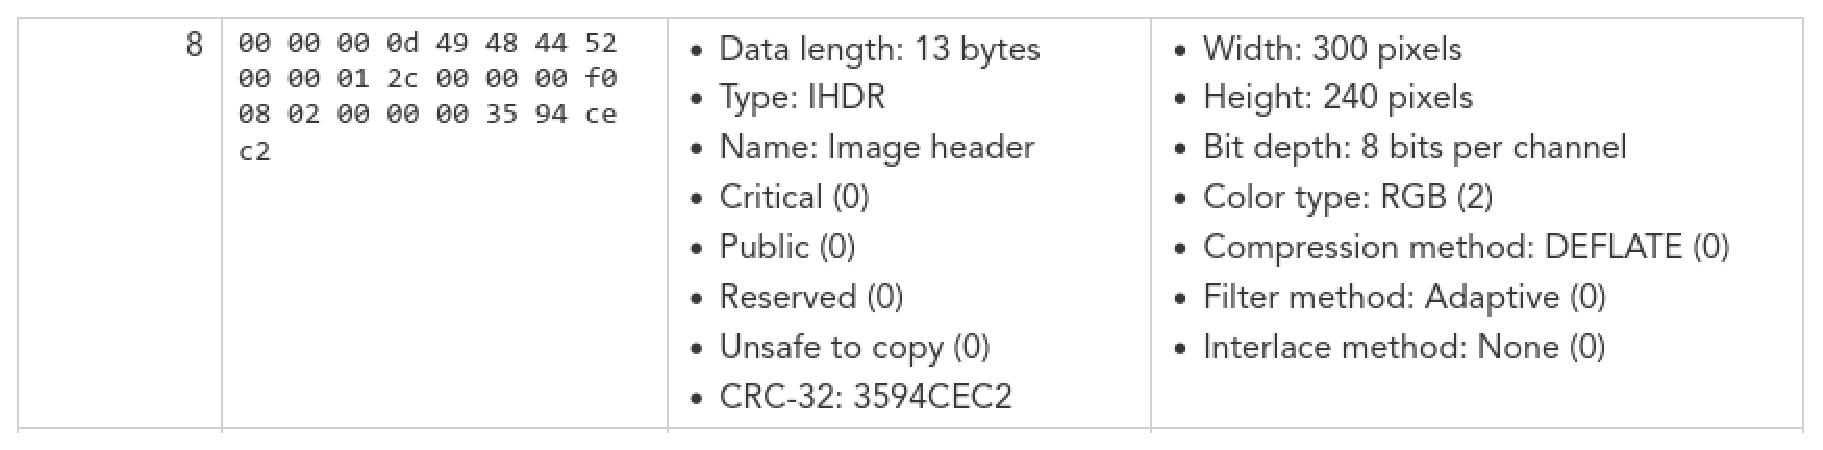
\includegraphics[width=1\textwidth]{img/png_ihdr.eps}
Chunk indispensable et doit être en premier qui contient les méta données du fichier PNG tels que la largeur, la longueur, la taille d'un canal de couleur (8 bits en PNG-8), méthode de compression, etc.


\subsubsection{IDAT chunk (Image data)}
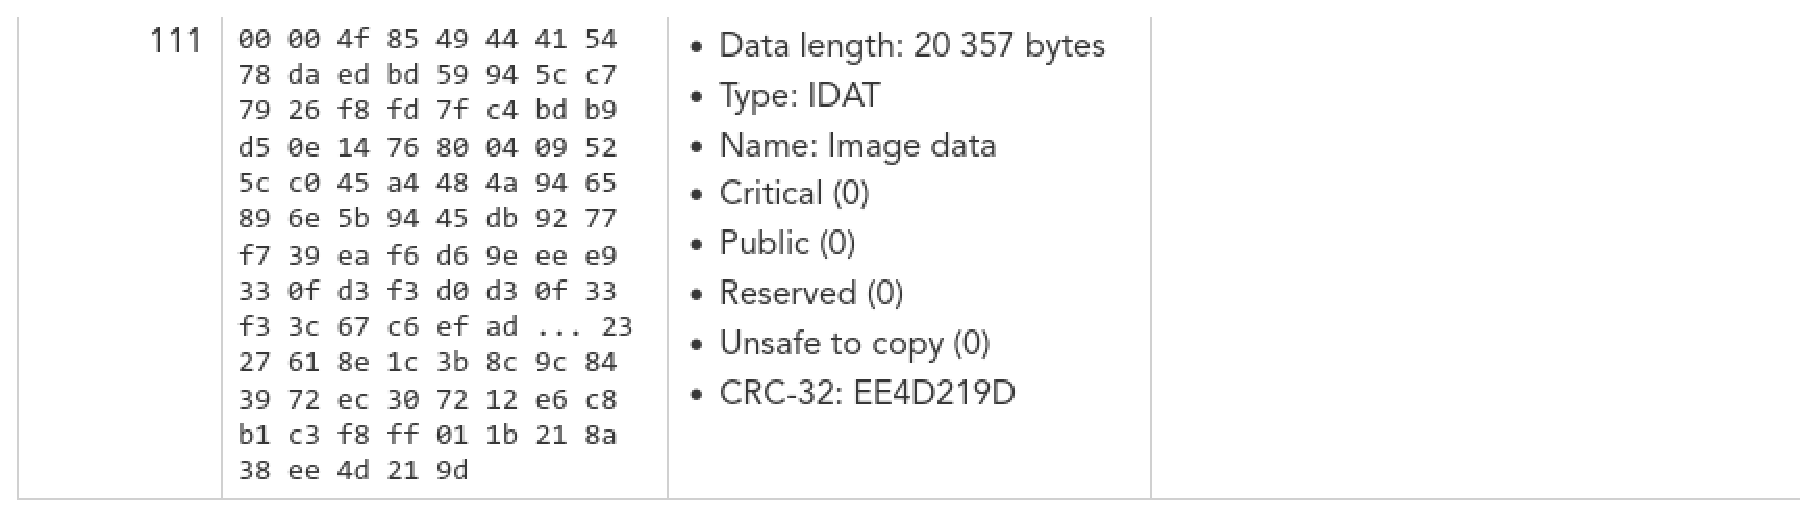
\includegraphics[width=1\textwidth]{img/png_idat.eps}
Chunk contenant les pixels de l'image. Il peut y avoir plusieurs chunk IDAT et peut être compressé si un algorithme de compression est mentionné dans le chunk IHDR. C'est principalement ce chunk que nous allons utiliser.


\subsubsection{IEND chunk}
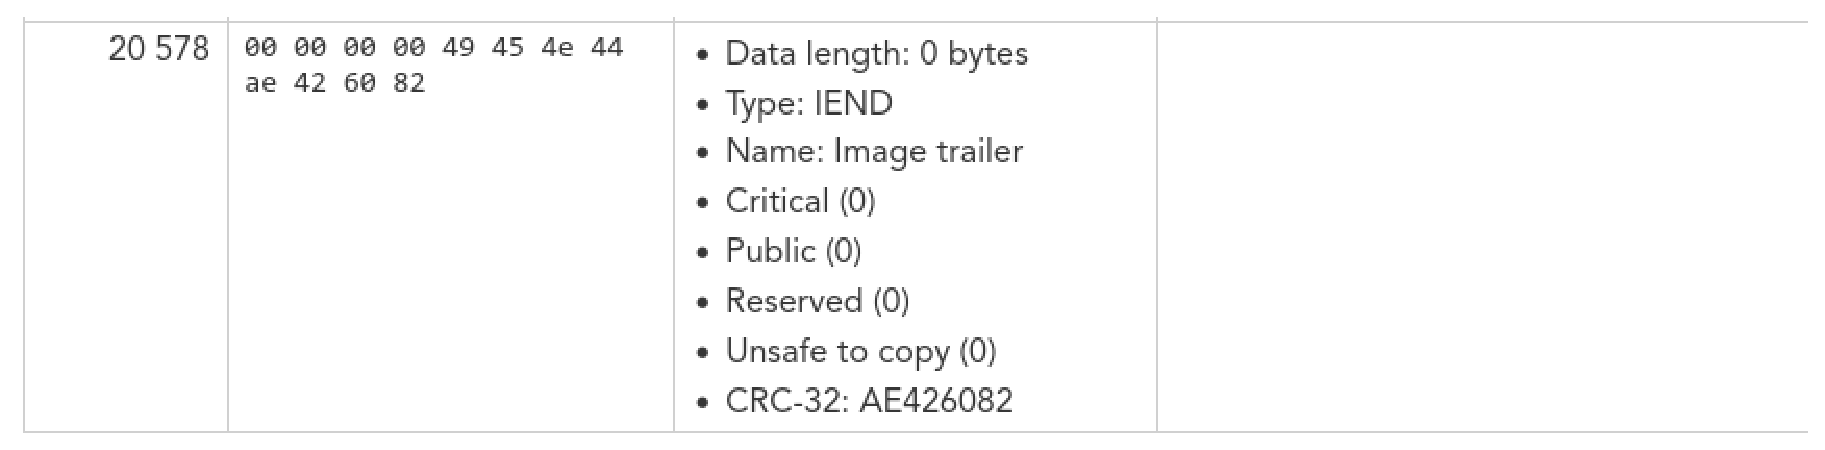
\includegraphics[width=1\textwidth]{img/png_iend.eps}
Chunk marquant la fin du fichier PNG. Il doit être placé à la fin et contient une section data vide.
\newline
D'autres chunks peuvent exister pour contenir d'autres informations facultatives tels que la transparence, les méta données (date de création, modification, etc.), la pallette de couleurs, etc.

\subsection{Structure du segment IDAT}
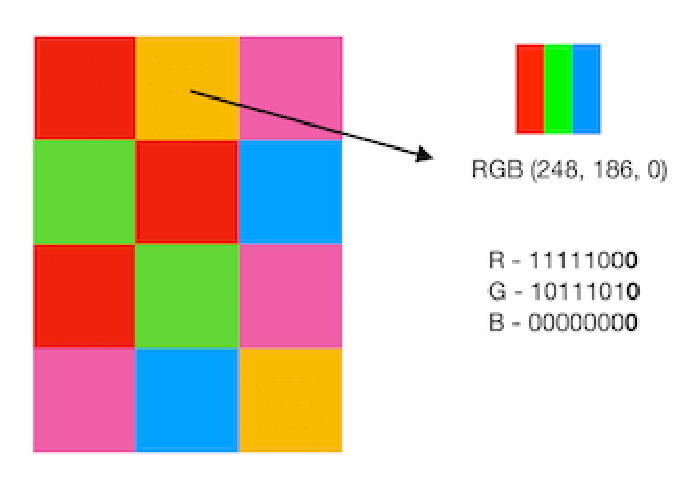
\includegraphics[width=1\textwidth]{img/RGB-png-bit-pixel-mode.eps}
Ici, je vais considérer que nous utillisons une image PNG sans compression où les pixels sont représentés par le type true color. Deux autres type existent (grayscale et indexed color) mais je ne m'attarderai pas dessus.
\newline
Dans la section données du segment IDAT, les pixels sont allignés l'un à la suite de l'autre. Chacun des pixels est composé de 3 canaux (rouge, vert et bleu) pour représenter la couleur de ce pixel. Chaque ligne de pixels est d'une longeur définie par le segment IHDR.
\newline
Un pixel d'une image PNG-8 a donc une taille de 3 octets et permet d'avoir 256³ couleurs différentes.
\subsection{LSB sur PNG}
L'idée de la stéganographie least significant bit est d'utiliser le bit de poids faible des canaux d'un pixel pour insérer des données.
\newline
Voici un exemple pour mieux comprendre :
\newline
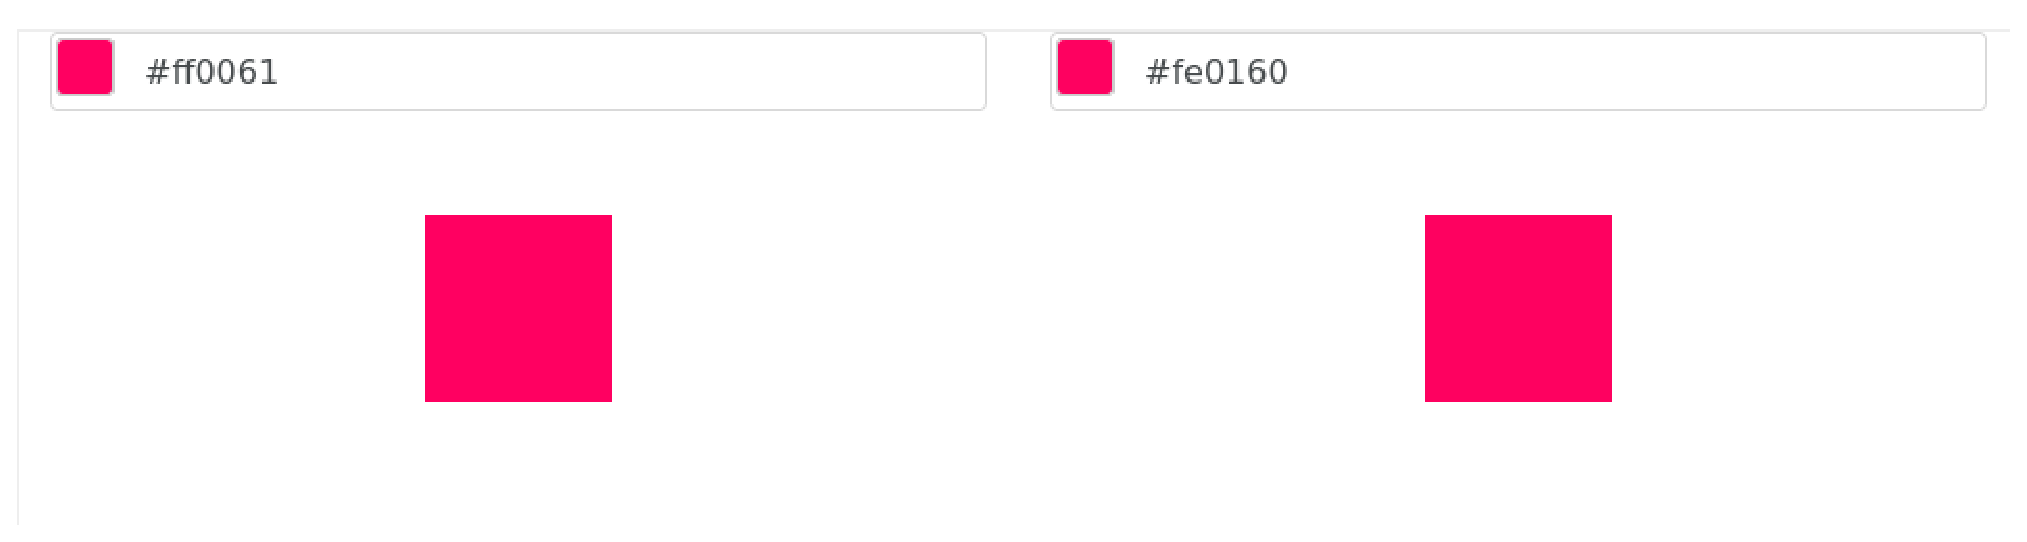
\includegraphics[width=1\textwidth]{img/color_comparaison.eps}
Ici, nous avons 2 couleurs. Une couleur de référence (à gauche) et une couleur où j'ai inversé le bit de poids faible des 3 canaux de couleur.
\newline
La différence est (quasi) invisible à l'oeil nu et le fait qu'un pixel soit de taille très petite rend l'impossibilité de détecter la différence de couleur, en tant qu'humain.
\newline
\newline
L'idée est donc de stocker des données binaires dans ces bits de poids faible. Exemple :
\newline
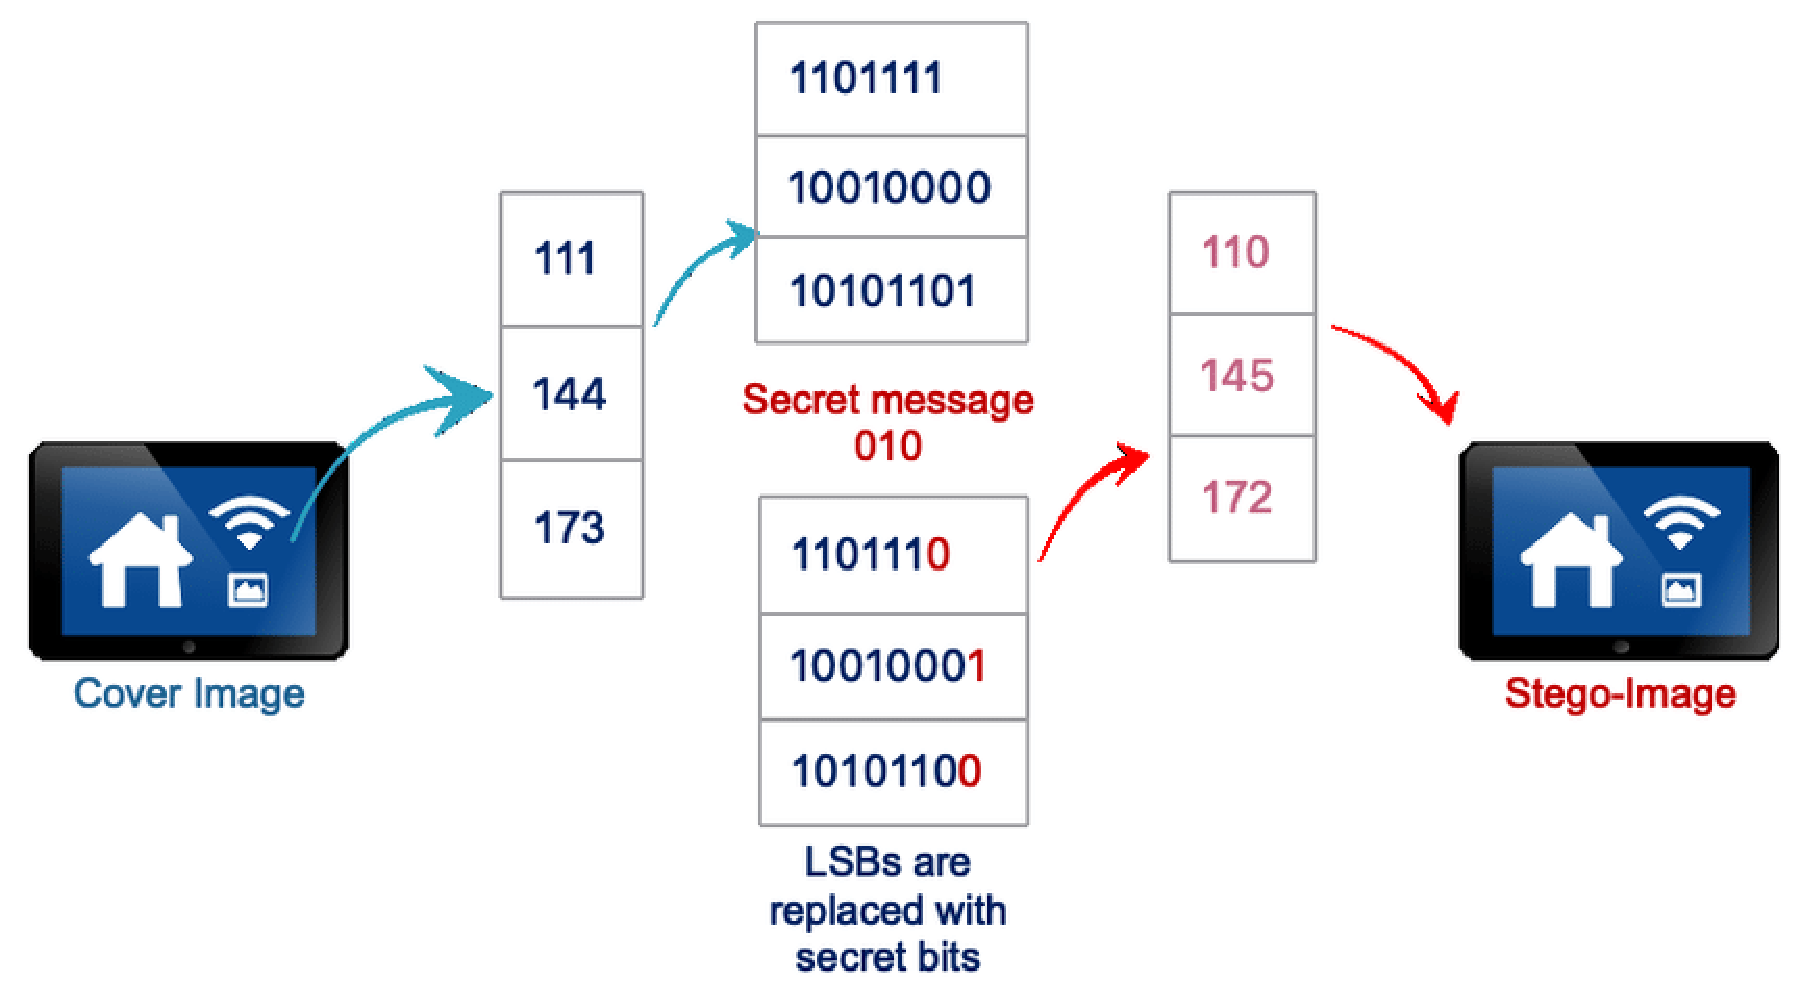
\includegraphics[width=1\textwidth]{img/LSB-image-steganography.eps}